\chapter{Feature Use and Ranking Results}
\label{app:featureUse}

\begin{figure}[htp]
\centering
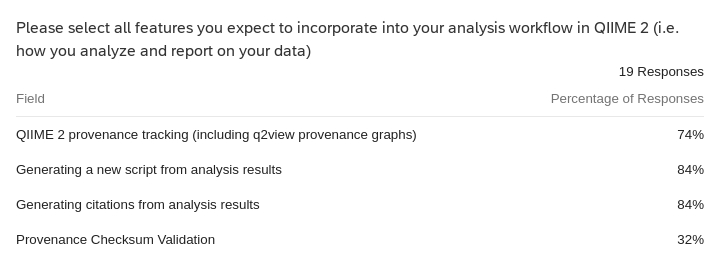
\includegraphics[width=\textwidth]{figures/feature_use.jpg}
\end{figure}

\begin{figure}[htp]
\centering
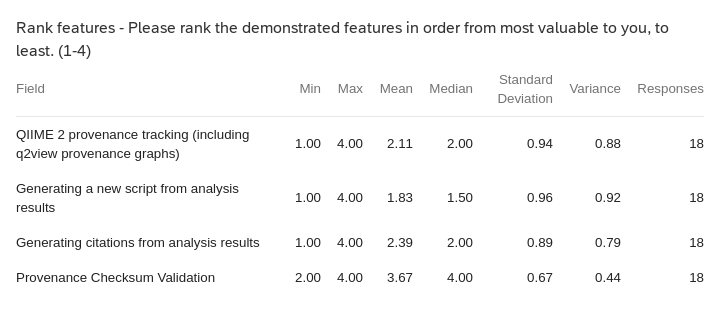
\includegraphics[width=\textwidth]{figures/feature_ranking.jpg}
\end{figure}